
\section{Results}
    \subsection{Quantitative Insights}\label{app:quantitative_insights}
        \subsubsection{Perceived User Experience}
        
        
        
        Figure~\ref{fig:ueq-distribution} presents participants' response to the individual item of the questionnaire which confirms that the \ac{CA} was easy to learn, easy to use, understandable (perspicuity); friendly (attractiveness) and well organized (efficiency).
            \begin{figure}[t]
                \centering
                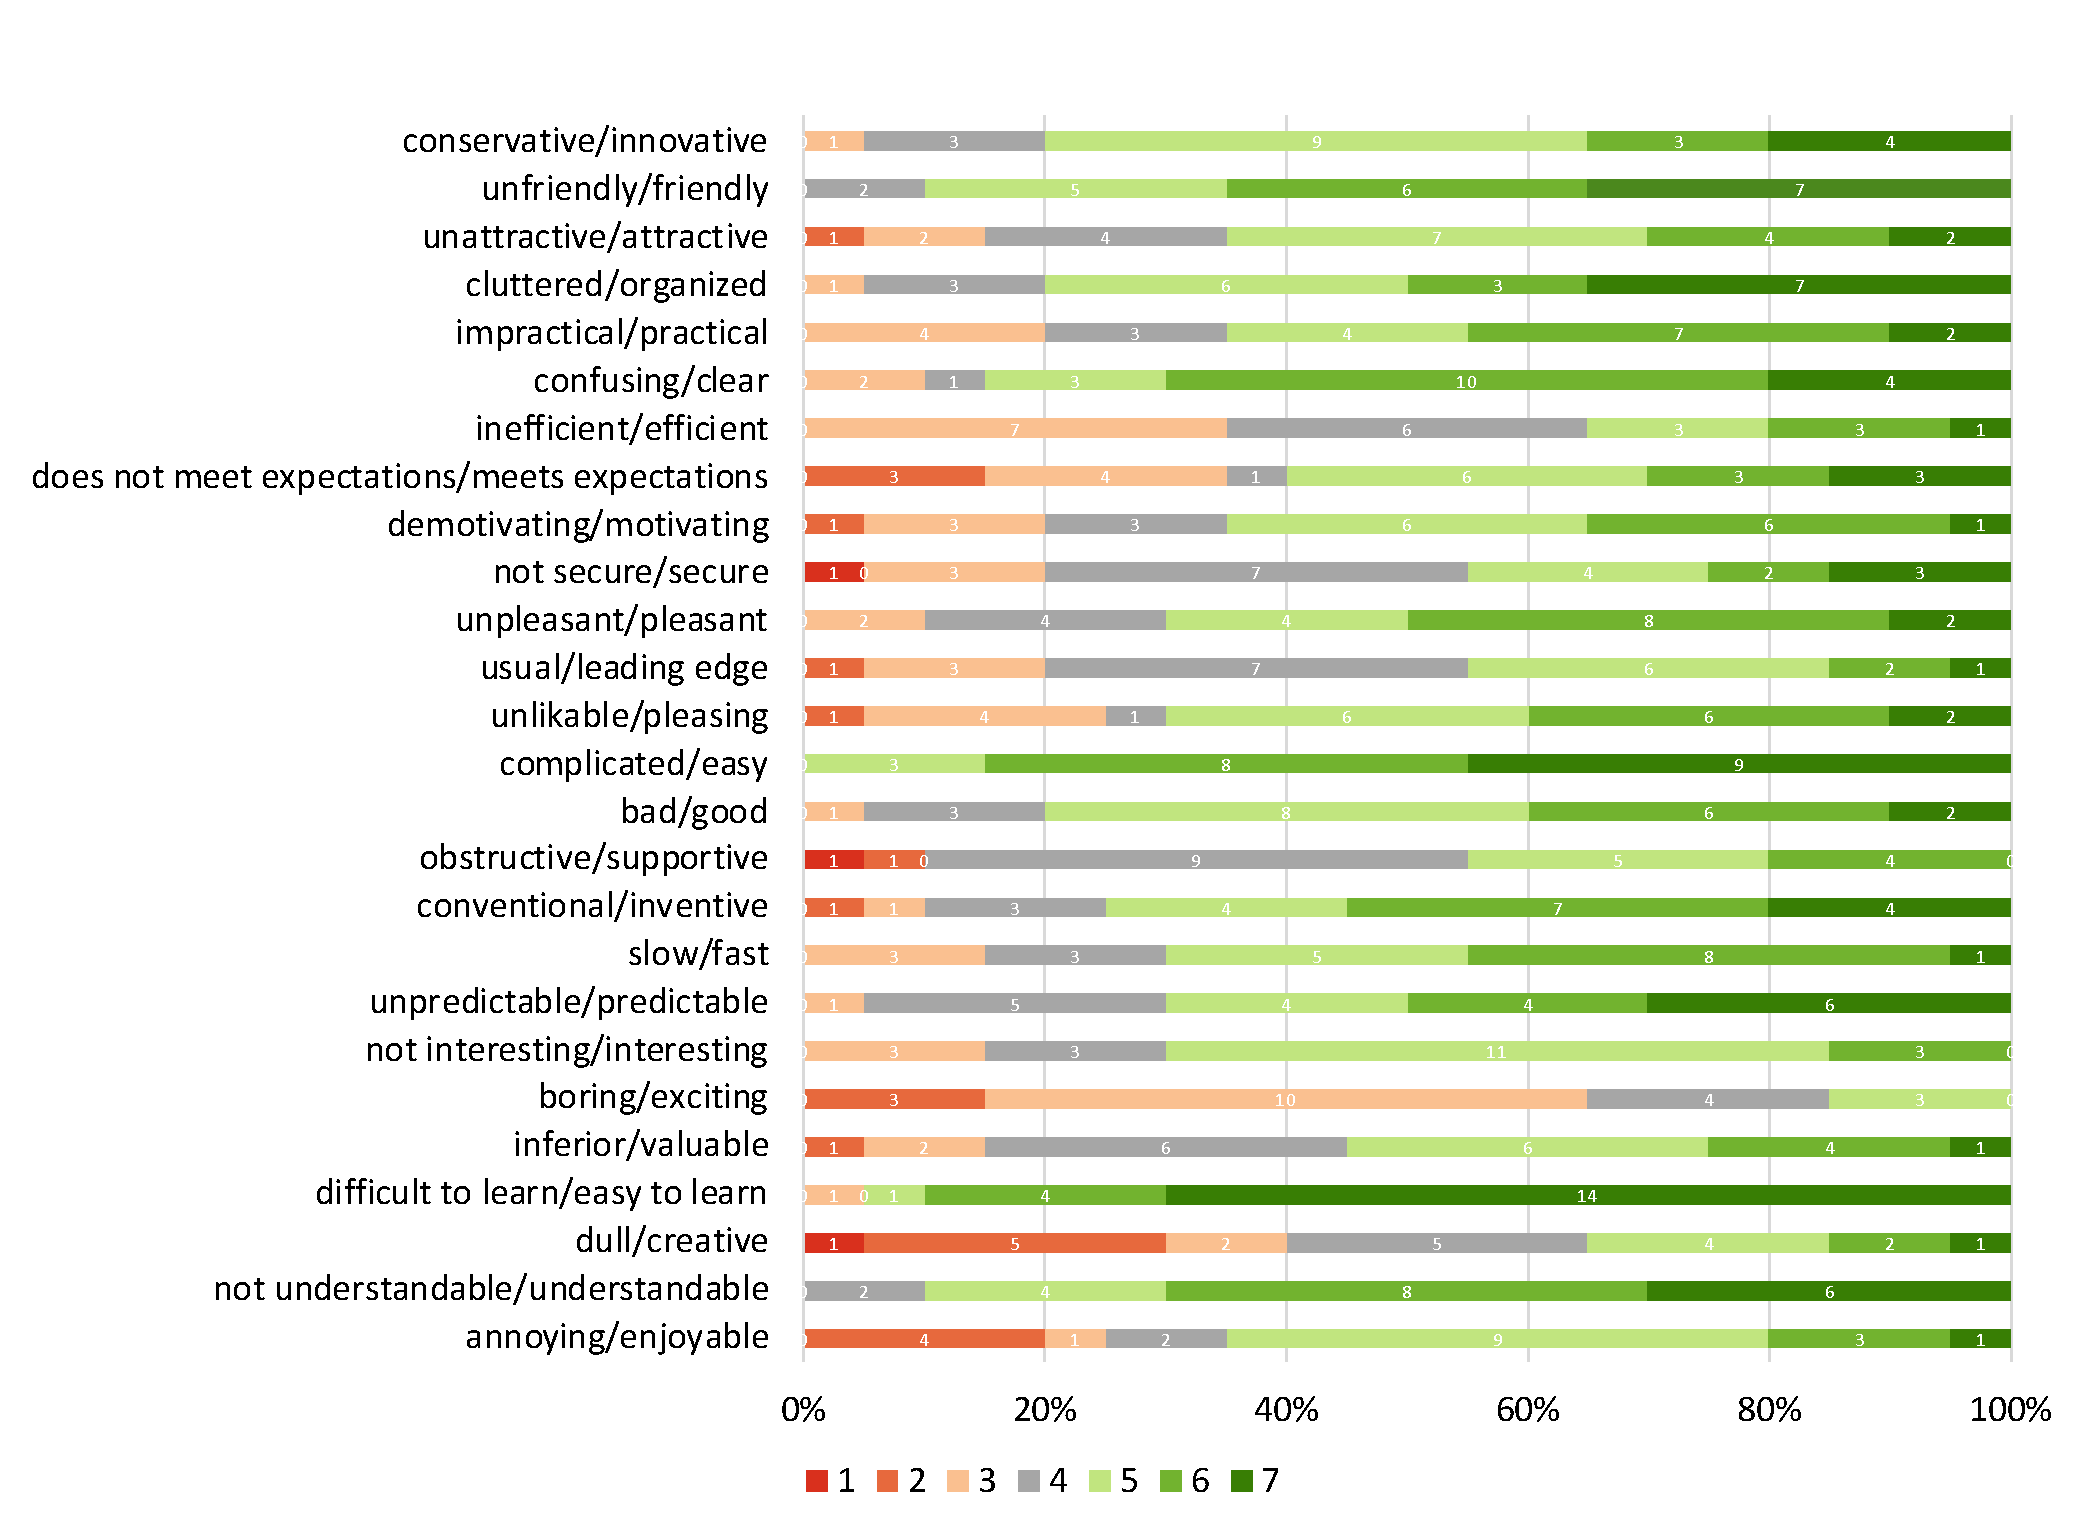
\includegraphics[clip, trim=0cm 0cm 0.25cm 0.25cm, width=\textwidth]{figures/ueq-distribution.pdf}
                \caption{Distribution of UEQ Answers per item (n=20). Labels 1 to 7 represent the spectrum of user's gradations between the opposite attributes of \acl{app} as such 1 denotes user's strong agreement with the negative attribute, 7 reflects positive impression and 4 indicates neutral sentiment. For example, users' response 1 to UEQ item `conservative/innovative' means their agreement that the system is conservative, 7 indicates that the system is innovative, and 4 represents users' neutral feedback. Annotations within the distribution represent the frequency of users' score.}
                \label{fig:ueq-distribution}
            \end{figure}
        
        Table \ref{tab:ueq_summary} shows the statistical summary of the participants' response to \ac{UEQ} scale.
        
        
                \begin{table}[t]
                \centering
                \caption{Statistical summary of the \ac{UEQ} scores. Confidence intervals (p=0.05) per scale.}
                \begin{tabular}{p{2cm} p{1cm} p{2cm} p{1cm} p{2cm} p{2cm} p{1.25cm}}
                    \toprule
                    \textbf{Scale}	& \textbf{Mean}	& \textbf{Std. Dev.}	& \textbf{N}	    & \textbf{Confidence}	& \multicolumn{2}{l}{\textbf{Confidence Interval}}\\
                    \midrule
                    Attractiveness	& 1.092	& 1.015	    & 20	& 0.445	        & 0.647	    & 1.537\\
                    Perspicuity	    & 2.088	& 0.749	    & 20	& 0.328	        & 1.759	    & 2.416\\
                    Efficiency	    & 0.975	& 0.773	    & 20	& 0.339	        & 0.636	    & 1.314\\
                    Dependability	& 0.738	& 0.837	    & 20	& 0.367	        & 0.371	    & 1.104\\
                    Stimulation	    & 0.375	& 0.817	    & 20	& 0.358	        & 0.017	    & 0.733\\
                    Novelty	        & 0.713	& 0.878	    & 20	& 0.385	        & 0.328	    & 1.097\\
                    \bottomrule
                \end{tabular}
                \label{tab:ueq_summary}
            \end{table}
        
        % \begin{figure}
        %     \centering
        %     \centering
        %     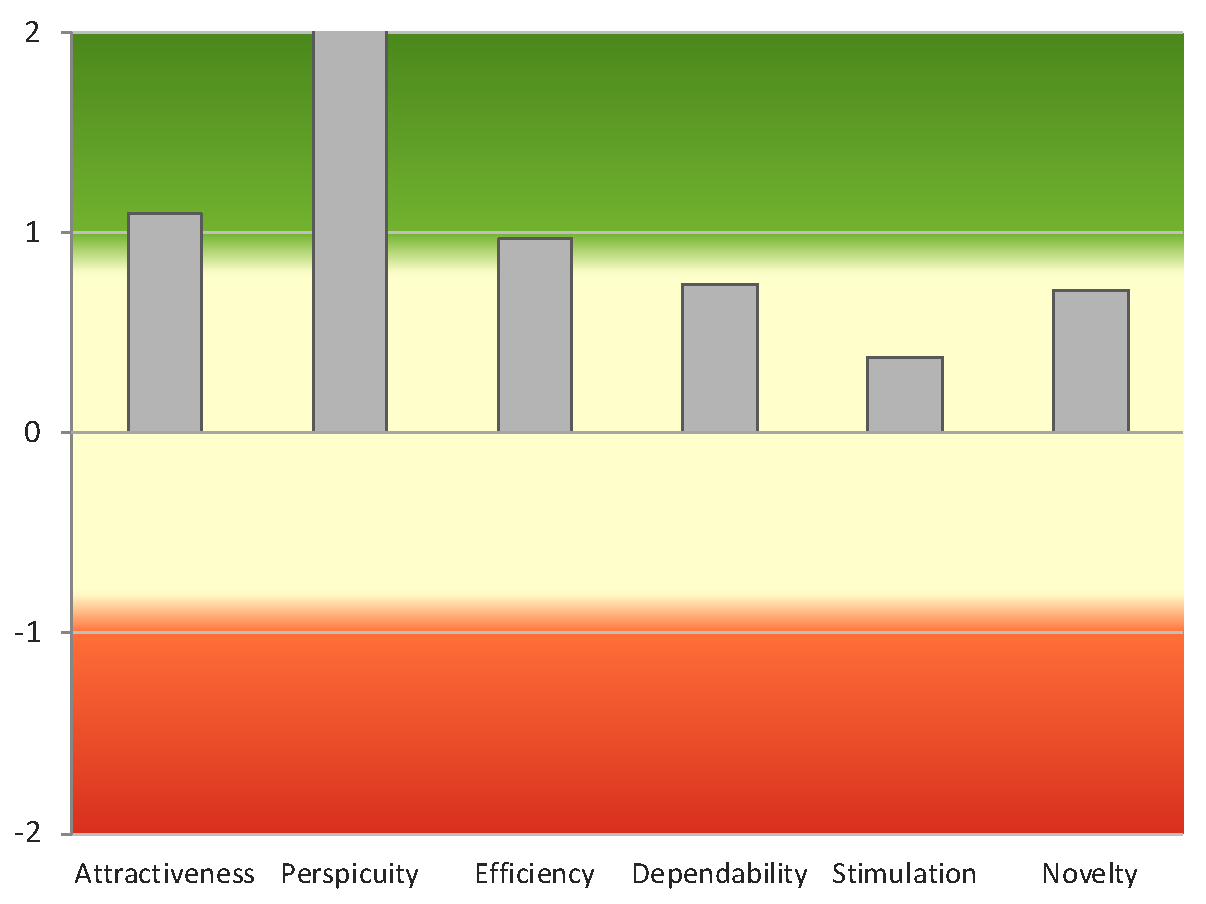
\includegraphics[width=0.75\textwidth]{figures/ueq-mean.pdf}
        %     \captionof{figure}{Participant's mean \ac{UEQ} scores aggregated into six dimensions attractiveness, perspicuity, efficiency, dependability, stimulation and novelty}
        %     \label{fig:ueq-mean}
        % \end{figure}
        
        Figure~\ref{fig:ueq-benchmark} illustrates the \ac{CA}'s \ac{UEQ} score compared to the benchmark data. The figure shows that the \ac{CA} is rated `excellent' for perspicuity which means that the rating is in the range of the 10\% of the best results in the benchmark data. Attractiveness, efficiency, and novelty were rated as `below average' which means 50\% of the results in the benchmark are better than the result for the evaluated system and 25\% of the results are worse. Finally, dependability and stimulation were rated as `bad' meaning that the the system is rated in range of the 25\% worst results in the benchmark data.
        \begin{figure}
            \centering
            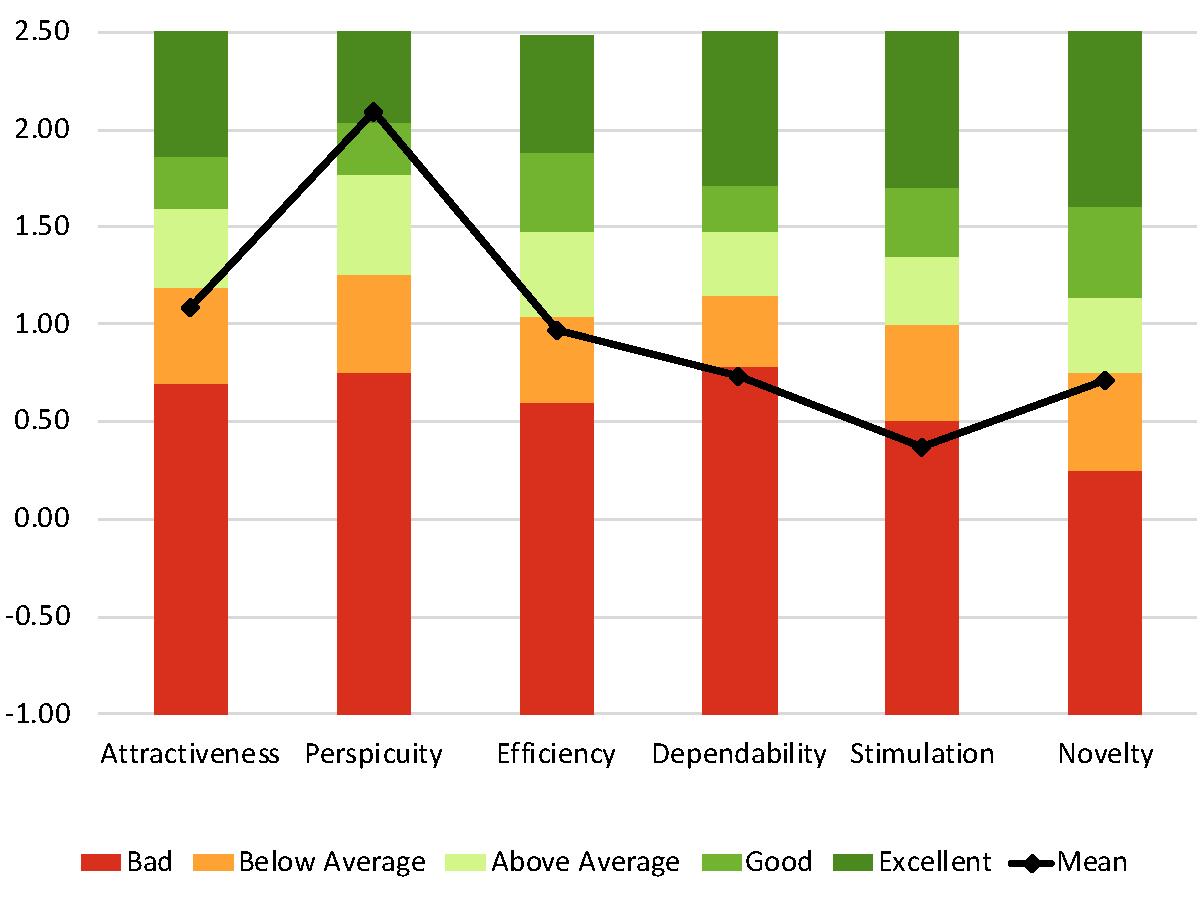
\includegraphics[width=0.7\textwidth]{figures/ueq-benchmark.pdf}
            \captionof{figure}{Comparison of the users scores for \acl{app} in each \ac{UEQ} dimension with the benchmark.
            }
            \label{fig:ueq-benchmark}
        \end{figure}
        
        
        The internal consistency of the \ac{UEQ} dimensions measured by Cronbach-Alpha in our evaluation resulted sufficient in terms of attractiveness ($\alpha = 0.89$), perspicuity ($\alpha = 0.76$) and stimulation ($\alpha = 0.73$). Whereas, the Cronbach-Alpha values for efficiency ($\alpha = 0.44$), dependability ($\alpha = 0.29$) and novelty ($\alpha = 0.57$) indicate poor internal consistency suggesting that the several participants might have interpreted the questions differently in the given context.
            
            
        
            
        

        

        




